\chapter{\IfLanguageName{dutch}{Stand van zaken}{State of the art}}
\label{ch:stand-van-zaken}

% Tip: Begin elk hoofdstuk met een paragraaf inleiding die beschrijft hoe
% dit hoofdstuk past binnen het geheel van de bachelorproef. Geef in het
% bijzonder aan wat de link is met het vorige en volgende hoofdstuk.

% Pas na deze inleidende paragraaf komt de eerste sectiehoofding.

%Dit hoofdstuk bevat je literatuurstudie. De inhoud gaat verder op de inleiding, maar zal het onderwerp van de bachelorproef *diepgaand* uitspitten. De bedoeling is dat de lezer na lezing van dit hoofdstuk helemaal op de hoogte is van de huidige stand van zaken (state-of-the-art) in het onderzoeksdomein. Iemand die niet vertrouwd is met het onderwerp, weet nu voldoende om de rest van het verhaal te kunnen volgen, zonder dat die er nog andere informatie moet over opzoeken \autocite{Pollefliet2011}.

%Je verwijst bij elke bewering die je doet, vakterm die je introduceert, enz. naar je bronnen. In \LaTeX{} kan dat met het commando \texttt{$\backslash${textcite\{\}}} of \texttt{$\backslash${autocite\{\}}}. Als argument van het commando geef je de ``sleutel'' van een ``record'' in een bibliografische databank in het Bib\LaTeX{}-formaat (een tekstbestand). Als je expliciet naar de auteur verwijst in de zin, gebruik je \texttt{$\backslash${}textcite\{\}}.
%Soms wil je de auteur niet expliciet vernoemen, dan gebruik je \texttt{$\backslash${}autocite\{\}}. In de volgende paragraaf een voorbeeld van elk.

%\textcite{Knuth1998} schreef een van de standaardwerken over sorteer- en zoekalgoritmen. Experten zijn het erover eens dat cloud computing een interessante opportuniteit vormen, zowel voor gebruikers als voor dienstverleners op vlak van informatietechnologie~\autocite{Creeger2009}.

% Te beschrijven in de stand van zaken
% Containers: Hoe werken ze en hoe worden ze gebruikt
% Docker: wat is het en waarvoor wordt het gebruikt?
% Container orkestratie: wat is het en waarom is het nodig
% Kubernetes: wat is het en waarvoor wordt het gebruikt?
% Security: veel voorkomende problemen, best practices
% Security tools: Welke zijn er en hoe werken ze

De stand van zaken of \textit{State of the art} geeft een beeld van de technologieën die worden overwogen voor dit onderzoek en op welke manieren ze kunnen toegepast worden om een antwoord te vinden op de onderzoeksvragen.

\section{Containers}
In dit hoofdstuk zal uitgelegd worden wat containers zijn, hoe ze werken en waarvoor ze worden gebruikt.

Containers bieden veel voordelen vergeleken met normale virtuele machines (vm's). Ze kunnen snel opgezet worden en zijn gemakkelijk om te configureren terwijl virtuele machines vaak groot en traag zijn. Containers zijn pakketten waarin een applicatie verpakt zit, samen met al zijn benodigde bibliotheken en afhankelijkheden. Hierdoor kunnen ze vlot van de ene omgeving naar de andere worden overgezet zonder dat er extra configuratie nodig is \autocite{Education2019}. Containers maken gebruik van een vorm van besturingssysteem virtualisatie om processen te isoleren van het host besturingssysteem en zo ook het CPU gebruik en hoeveelheid RAM geheugen van die processen te controleren.\autocite{Docker2018}

Containers hebben geen eigen besturingssysteem nodig, alle containers delen 1 gezamenlijke 'runtime engine'. Een runtime engine is de laag die verantwoordelijk is voor de communicatie tussen het besturingssysteem van de host machine en de containers zelf. De meeste gebruikte runtime engine is de 'Docker Engine'\footnote{https://docs.docker.com/engine/}.

\subsection{Container vs. virtuele machine}
Bij traditionele virtuele machines virtualiseert een 'hypervisor' de fysieke hardware. De hypervisor regelt het resource gebruik tussen de verschillende vm's en zorgt ervoor dat de hardware van de 'host' (de fysieke hardware waar de hypervisor op geinstaleed is) eerlijk verdeelt wordt. Elke vm heeft zijn eigen volwaardig besturingssysteem, wat ervoor zorgt dat ze zeer veel resources gebruiken en vaak traag zijn. In plaats van de onderliggende hardware te visualiseren containers het besturingssysteem (meestal is dit Linux), zodat elke individuele container enkel de applicatie en de bijhorende bibliotheken en afhankelijkheden bevat \autocite{Education2020}.

\begin{figure}[ht]
    \centering
    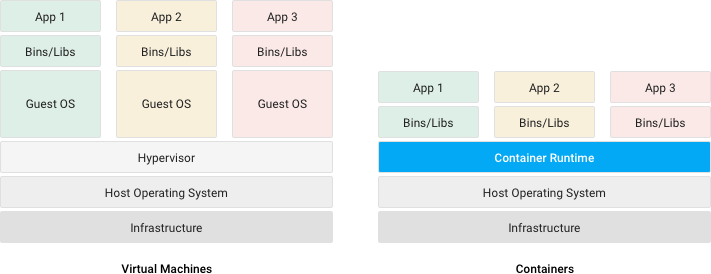
\includegraphics[width=\linewidth]{img/container-vs-vm.png}
    \caption{Container vs. virtuale machine \autocite{Google2016}}
    \label{fig:example}
\end{figure}


\subsection{Waarvoor worden containers gebruikt}
Containers zijn zeer veelzijdig en kunnen in veel verschillende omstandigheden gebruikt worden. Docker\footnote{https://www.docker.com/} geeft enkele use cases waarvoor containers zeer geschikt zijn \autocite{Docker2021} :

\begin{itemize}
  \item \textit{Microservices}: Containers zijn klein en licht, waardoor ze goed passen bij microservice-architecturen waarin applicaties zijn opgebouwd uit vele, losjes gekoppelde en onafhankelijk services.
  \item \textit{Modernisering en migratie van applicaties}: Een van de meest voorkomende benaderingen voor het moderniseren van applicaties begint met het containeriseren ervan, zodat ze naar de cloud kunnen worden gemigreerd.
  \item \textit{Nieuwe ontwikkelaars snel inwerken}: Door gebruik te maken van containers verloopt het opzetten van een nieuwe lokale ontwikkelingsomgeving snel en vlot, waardoor de ontwikkelaars direct aan de slag kunnen
\end{itemize}


\section{Docker}
Hier zal uitgelegd worden wat docker is en hoe het ontstaan en gegroeid is.

\subsection{Hoe werkt docker}
Hier zal de werking van Docker uitgelegd worden, ook de verschillende technische termen die eigen zijn aan Docker zullen uitgelegd worden.

\section{Container orkestratie}
Hier zal uitgelegd worden wat container orkestratie is en waarvoor het gebruikt kan worden.

\subsection{Hoe werkt container orkestratie}
Hier zal de innerlijke werking van container orkestratie uitgelegd worden.

\section{Kubernetes}
Hier zal uitgelegd worden wat k8s is en hoe het werkt, ook de verschillende technische termen die eigen zijn aan k8s zullen uitgelegd worden.

\section{Security}
Hier word het security aspect van containers en container orkestratie besproken. (redelijk high level want kan ongeloofelijk complex worden)

\subsection{Meest voorkomende security problemen}
Hier worden de meest voorkomende security problemen opgelijst en worden ze kort besproken (Techinsche uitleg over hoe deze problemen onstaan)

\subsection{Hoe een container cluster beveiligen}
Uitleg over hoe een container cluster beveiligt kan worden (Best practices en security tools) + uitleg over ingebouwde security features.

\section{Security tools}
Hier worden enkele security tools opgeslijst en hun werking kort besproken.